\begin{question}
True or false: the two level surfaces $f(x,y,z)=3$ and $f(x,y,z)=5$ of the function $f(x,y,z)=2x^2 + y^3 + z^4$ do not intersect at any point in space?
\end{question}

\begin{solution}
True.

If the level surfaces did intersect, say at $(a,b,c)$, then we'd have $f(a,b,c)=3$ and at the same time $f(a,b,c)=5$; but this is impossible, since $f$ is a function (one output only).
\end{solution}

\begin{question}
The following figure shows contour diagrams of $f(x,y)$ (dashed lines) and $g(x,y)$ (solid lines). Plot 3 points, where $f(x,y) = g(x,y)$.

\begin{center}
\begin{tikzpicture}[scale=1.8]
  \clip[draw] (0,0) rectangle (3.5, 3.5);

  % Solid lines
  \foreach \xa/\xb/\yb/\xl in {1 / 3.4 / 1   / 2, 
                               2 / 3.1 / 1.7 / 4, 
                               3 / 2.8 / 2.3 / 6, 
                               4 / 2.4 / 3.1 / 8, 
                               5 / 1.8 / 4   / 10, 
                               6 / 1.2 / 5   / 12, 
                               8 / 0.5 / 6   / 14}{

    % Straight lines -- solid and black
    \draw[name path=w] (0,\xa) -- node[midway,fill=white]{$\xl$} 
                       (\xa,0);

    % Parabolas -- dashed and blue
    \draw[dashed, blue, name path=p] (\xb-6,3.5-\xb+\yb) 
      parabola bend (\xb,3.5-\xb) (\xb+6,3.5-\xb+\yb);

    \path[name path=v] (1.8,0) -- (1.8,3.5);
    \path[name intersections={of=v and p}];
    \coordinate (A) at (intersection-1);
    \node[blue, fill=white] at (A) {$\xl$};
  };
\end{tikzpicture}
\end{center}
\end{question}

\begin{solution}
The points are marked in the figure below.
\begin{center}
\begin{tikzpicture}[scale=1.8]
  \clip[draw] (0,0) rectangle (3.5, 3.5);

  % Solid lines
  \foreach \xa/\xb/\yb/\xl in {1 / 3.4 / 1   / 2, 
                               2 / 3.1 / 1.7 / 4, 
                               3 / 2.8 / 2.3 / 6, 
                               4 / 2.4 / 3.1 / 8, 
                               5 / 1.8 / 4   / 10, 
                               6 / 1.2 / 5   / 12, 
                               8 / 0.5 / 6   / 14}{

    % Straight lines -- solid and black
    \draw[name path=w] (0,\xa) -- node[midway,fill=white]{$\xl$} 
                       (\xa,0);

    % Parabolas -- dashed and blue
    \draw[dashed, blue, name path=p] (\xb-6,3.5-\xb+\yb) 
      parabola bend (\xb,3.5-\xb) (\xb+6,3.5-\xb+\yb);

    \path[name path=v] (1.8,0) -- (1.8,3.5);
    \path[name intersections={of=v and p}];
    \coordinate (A) at (intersection-1);
    \node[blue, fill=white] at (A) {$\xl$};
    
    % Solution circles
    \path[name intersections={of=w and p}];
    \coordinate (B) at (intersection-1);
    \draw[fill=white] (B) circle (0.08);
  };
\end{tikzpicture}
\end{center}
\end{solution}

\begin{question}
Consider the function $f(x,y) = 3y^2 - 4x^3$. Suppose you are standing on the surface at the point where $x=3$ and $y=-1$. If you start to move on the surface parallel to the $y$-axis in the direction of increasing $y$, does your height increase or decrease?
\end{question}

\begin{solution}
With $x=3$ fixed, our height, when moving parallel to the $y$-axis, will be described by the function
\[
g(y) = f(3,y) = 3y^2 - 108\,.
\]
The graph of $g$ is a parabola, shifted downwards by 108, whose graph is sketched below. Thus, if we increase $y$, starting at $y=-1$, the value of $z$ will decrease.

\begin{center}
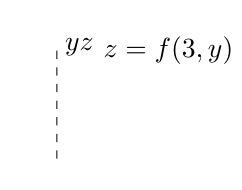
\begin{tikzpicture}[scale=0.9375, baseline=0]
 \def\scale{0.9375}

 % \draw[coordinate grid, step=0.5] (-2, -2) grid (2, 2);
 \drawxaxis[$y$]{-2}{2}
 \drawyaxis[$z$]{-2}{2}

 \draw plot[parametric, domain=-2:2, samples=100] function {t, t**2-1.75}
   node[right] {$z = f(3,y)$};

 \coordinate (a) at (-0.5, {0.25-1.75});
 \draw[dashed] (-0.5, 0) -- (a);
 \drawpoint{(a)}

 \drawxlabels{-0.5/-1}

\end{tikzpicture}
\end{center}
\end{solution}

\begin{question}
Determine which surface (1) -- (3) corresponds to which defining equation (a) -- (c).
\begin{tasks}(3)
\task
$x^2 + y^2 = 1$
\task
$x^2 + z^2 = 1$
\task
$y^2 + z^2 = 1$
\end{tasks}

\begin{center}
\begin{tabu} to \linewidth {X[1,c] X[1,c] X[1,c]}
\asyinclude[width=4cm]{asy/match_cylinder_x.asy} &
\asyinclude[width=4cm]{asy/match_cylinder_y.asy} &
\asyinclude[width=3cm]{asy/match_cylinder_z.asy} \\
(1) & 
(2) & 
(3)
\end{tabu}
\end{center}
\end{question}

\begin{solution}
We have the following correspondences:

\begin{center}
\begin{tabu} to \linewidth {X[1,c] X[1,c] X[1,c]}
\asyinclude[width=4cm]{asy/match_cylinder_x.asy} &
\asyinclude[width=4cm]{asy/match_cylinder_y.asy} &
\asyinclude[width=3cm]{asy/match_cylinder_z.asy} \\
(1) -- (c) $y^2 + z^2 = 1$ & 
(2) -- (b) $x^2 + z^2 = 1$ & 
(3) -- (a) $x^2 + y^2 = 1$
\end{tabu}
\end{center}

We can use the method of missing variables to determine them: Note that each of the given equations omits one of the variables $x, y, z$. For example equation (a) omits $z$ and therefore the corresponding surface looks the same, when intersected with any plane $z=c$, where $c \in \R$ is a constant. Only Fig. (3) has this property. 

Similarly, equation (b) omits the variably $y$ and therefore all intersections of its surface with planes $y=c$ looks the same. Only Fig. (2) has this property. Finally, this leaves equation (c), which has to match Fig. (1).
\end{solution}

\begin{question}
Determine which surface (1) -- (3) corresponds to which defining equation (a) -- (c).
\begin{tasks}(3)
\task
$\frac x 4 = y^2 + z^2$
\task
$\frac y 4 = x^2 + z^2$
\task
$\frac z 4 = x^2 + y^2$
\end{tasks}

\begin{center}
\begin{tabu} to \linewidth {X[1,c] X[1,c] X[1,c]}
\asyinclude[width=3.5cm]{asy/match_paraboloid_z.asy} &
\asyinclude[width=3.5cm]{asy/match_paraboloid_x.asy} &
\asyinclude[width=4cm]{asy/match_paraboloid_y.asy} \\
(1) & 
(2) & 
(3)
\end{tabu}
\end{center}
\end{question}

\begin{solution}
We have the following correspondences:

\begin{center}
\begin{tabu} to \linewidth {X[1,c] X[1,c] X[1,c]}
\asyinclude[width=3.5cm]{asy/match_paraboloid_z.asy} &
\asyinclude[width=3.5cm]{asy/match_paraboloid_x.asy} &
\asyinclude[width=4cm]{asy/match_paraboloid_y.asy} \\
(1) -- (c) $\frac z 4 = x^2 + y^2$ & 
(2) -- (a) $\frac x 4 = y^2 + z^2$ & 
(3) -- (b) $\frac y 4 = x^2 + z^2$
\end{tabu}
\end{center}

Note that each of the given equations describes the graph of a function. For example, equation (a) can be regarded as describing the graph of a function $x = f(y,z)$, where $y$ and $z$ are the independent variables and $x$ is the dependent variable. What is the function? In this case $f(y,z) = 4(y^2 + z^2)$. Only Fig. (2) is the graph of a function with $y$, $z$ as independent variables, because only in Fig. (2) is the $x$-coordinate of a point on the surface uniquely determined by the $y$- and $z$-coordinates.

Similarly, equation (b) can be viewed as the graph of a function $y = f(x,z)$ with $x$, $z$ as the independent variables. Only in Fig. (3) can $y$ be viewed as a function of the other variables. Finally, this leaves equation (c), which has to match Fig. (1).
\end{solution}

\begin{question}
Determine which surface (1) -- (3) corresponds to which defining equation (a) -- (c).
\begin{tasks}(3)
\task
$z = y^2-x^2$
\task
$z = 2x^2$
\task
$z = 2y^2$
\end{tasks}

\begin{center}
\begin{tabu} to \linewidth {X[1,c] X[1,c] X[1,c]}
\asyinclude[width=3.5cm]{asy/match_parabola_xz.asy} &
\asyinclude[width=4cm]{asy/match_parabola_xz_2.asy} &
\asyinclude[width=3.5cm]{asy/match_saddle.asy} \\
(1) & 
(2) & 
(3)
\end{tabu}
\end{center}
\end{question}

\begin{solution}
We have the following correspondences:

\begin{center}
\begin{tabu} to \linewidth {X[1,c] X[1,c] X[1,c]}
\asyinclude[width=3.5cm]{asy/match_parabola_xz.asy} &
\asyinclude[width=4cm]{asy/match_parabola_xz_2.asy} &
\asyinclude[width=3.5cm]{asy/match_saddle.asy} \\
(1) -- (b) $z = 2x^2$ & 
(2) -- (c) $z = 2y^2$ & 
(3) -- (a) $z = y^2 - x^2$
\end{tabu}
\end{center}

Only in equation (a) can $z$ -- because of the presence of $-x^2$ -- take negative values. Therefore equation (a) has to correspond to Fig. (3). This leaves equations (b) and (c). To distinguish them we can look at their level sets. For $z=2x^2$, the level sets $z=c$ take the form $2x^2 = c$. They describe the two lines
\[
x = \frac 12 \sqrt{2c} \text{ and } x = -\frac 12 \sqrt{2c}\,.
\]
The level sets in Fig. (1) are lines of the form $x=k$ with some $k \in \R$, while the level sets in Fig. (2) are lines of the form $y=k$. Thus (b) corresponds to (1) and (c) to (2).
\end{solution}

\begin{question}
Match the function with its graph and justify your reasoning.
\begin{tasks}(2)
\task
$f(x,y) = \sin x - \sin y$
\task
$f(x,y) = \sin (x-y)$
\end{tasks}

\begin{center}
\begin{tabu} to \linewidth {X[1,c] X[1,c]}
\asyinclude[width=6.8cm]{asy/match_sin_1.asy} &
\asyinclude[width=6.8cm]{asy/match_sin_2.asy} \\
(1) & 
(2)
\end{tabu}
\end{center}
\end{question}

\begin{solution}
We can distinguish the two functions by looking at the sections $y=k$ for $k \in \R$ a constant.
\begin{enumerate}
\item
For the function $f(x,y) = \sin x - \sin y$ these sections are $z = \sin x - \sin k$. In other words the graph $z = \sin x$ is shifted up and down as $y$ varies.
\item
For the function $f(x,y) = \sin(x-y)$ these sections are $z = \sin (x-k)$. In other words the graph $z = \sin x$ is shifted to the right and to the left as $y$ varies.
\end{enumerate}

So we conclude that the right correspondences are (1) -- (b) and (2) -- (a).
\end{solution}

\begin{question}
Describe the maximal domain of definition for each of the following functions.
\begin{tasks}(2)
\task
$f(x,y) = \displaystyle\frac{y}{x}$
\task
$f(x,y) = \displaystyle\frac{x+y}{x-y}$
\task
$f(x,y) = \displaystyle\frac{x+y}{x^2+y^2-1}$
\task
$f(x,y) = \sqrt{y - x^2}$
\task
$f(x,y) = \sqrt{x} \ln (y-\sin x)$
\task
$f(x,y) = \sqrt{y - \ln(-x)}$
\end{tasks}
\end{question}

\begin{solution}
We will denote by $D(f)$ the maximal domain of definition.
\begin{enumerate}
\item
The function can be defined everywhere, where $x \neq 0$. Therefore
\[
D(f) = \{ (x,y)\,:\, x \neq 0 \} = \R^2 \setminus \{ x = 0 \} \,;
\]
the domain consists of the whole plane except for the $y$-axis.
\item
The function can be defined everywhere, where $x - y \neq 0$. Therefore
\[
D(f) = \{ (x,y) \,:\, x \neq y \} = \R^2 \setminus \{ x=y \} \,;
\]
the domain consists of the whole plane except for those points lying on the line $x=y$.
\item
Here the denominator is $0$, when $x^2 + y^2 = 1$. Therefore
\[
D(f) = \{ (x,y) \,:\, x^2 + y^2 \neq 1 \} = \R^2 \setminus \{ x^2 + y^2 = 1\} \,;
\]
the domain conists of the whole plane except for the circle around the origin with radius 1.
\end{enumerate}

\begin{center}
\begin{figuretable}{3}
\begin{tikzpicture}[scale=1.25, baseline=0]
 \def\scale{1.25}

 \draw[coordinate grid, step=0.5] (-1.5, -1.5) grid (1.5, 1.5);
 \drawaxes{-1.5}{-1.5}{1.5}{1.5}

 \fill[pattern color=blue!30, pattern=north east lines] (-1.5, -1.5) |- (1.5, 1.5) |- cycle;
 \draw[draw=white, very thick] (0, -1.5) -- (0, 1.5);
 \draw[draw=black, dashed] (0, -1.5) -- (0, 1.5);

 \drawxlabels[nofill]{1/1}
 \drawylabels[nofill]{1/1}
\end{tikzpicture}
&
\begin{tikzpicture}[scale=1.25, baseline=0]
 \def\scale{1.25}

 \draw[coordinate grid, step=0.5] (-1.5, -1.5) grid (1.5, 1.5);
 \drawaxes{-1.5}{-1.5}{1.5}{1.5}

 \fill[pattern color=blue!30, pattern=north east lines] (-1.5, -1.5) |- (1.5, 1.5) |- cycle;
 \draw[draw=white, very thick] (-1.5, -1.5) -- (1.5,1.5);
 \draw[draw=black, dashed] (-1.5,-1.5) -- (1.5, 1.5);

 \drawxlabels[nofill]{1/1}
 \drawylabels[nofill]{1/1}
\end{tikzpicture}
&
\begin{tikzpicture}[scale=1.25, baseline=0]
 \def\scale{1.25}

 \draw[coordinate grid, step=0.5] (-1.5, -1.5) grid (1.5, 1.5);
 \drawaxes{-1.5}{-1.5}{1.5}{1.5}

 \fill[pattern color=blue!30, pattern=north east lines] (-1.5, -1.5) |- (1.5, 1.5) |- cycle;
 \draw[draw=white, very thick] (0,0) circle [radius=1];
 \draw[draw=black, dashed] (0,0) circle [radius=1];

 \drawxlabels[nofill]{1/1}
 \drawylabels[nofill]{1/1}
\end{tikzpicture} \\
(a) & (b) & (c)
\end{figuretable}
\end{center}

\begin{enumerate}[resume]
\item
For the square root to be well-defined we need the inequality $y - x^2 \geq 0$ to be satisfied. Therefore
\[
D(f) = \{ (x,y) \,:\, y \geq x^2 \}\,;
\]
the domain consists of the part of the plane, that lies on and above the parabola $y=x^2$.
\item
Here we need $x \geq 0$ for the square root to be well-defined and $y > \sin x$ to evaluate the logarithm. Note that one inequality is strict, while the other is not. Thus the domain is
\[
D(f) = \{ (x,y)\,:\, x \geq 0 \text{ and } y > \sin x \}\,;
\]
\item
To be able to evaluate $f(x,y)$ we need $-x > 0$ as well as $y - \ln(-x) \geq 0$ to be satisfied. These inequalities can be rewritten as
\[
D(f) = \{ (x,y) \,:\, x < 0 \text{ and } y \geq \ln(-x) \}\,.
\]
Note again, that one inequality is strict and the other is not.
\end{enumerate}

\begin{center}
\begin{figuretable}{3}
\begin{tikzpicture}[scale=1.25, baseline=(X.base)]
  \def\scale{1.25}
  \draw[coordinate grid, step=0.5] (-1.5,-1.5) grid (1.5,1.5);
  \node at (0,-1.5) (X) {};

  \drawaxes{-1.5}{-1.5}{1.5}{1.5}

  \clip (-1.5, -1.5) rectangle (1.5, 1.5);

  \fill[pattern color=blue!30, pattern=north east lines]
    plot[parametric, domain=-1.5:1.5, samples=100] function {t, t**2}
    -- cycle;

  \draw plot[parametric, domain=-1.5:1.5, samples=100] function {t, t**2};

  \drawxlabels[nofill]{1/1}
  \drawylabels[nofill]{1/1}
\end{tikzpicture}
&
\begin{tikzpicture}[scale=0.75, baseline=(X.base)]
 \def\scale{0.75}

 \draw[coordinate grid, xstep={pi/4}] (0, -2) grid ({3*pi/2}, 3);
 \node at (0,-2) (X) {};
 \drawaxes{0}{-2}{5}{3}

 \fill[pattern color=blue!30, pattern=north east lines]
   plot[domain={0:3*pi/2}, samples=100] function {sin(x)}
   |- (0, 3) -- cycle;

 \draw[draw=white, very thick] 
   plot[domain={0:3*pi/2}, samples=100] function {sin(x)};
 \draw[draw=black, dashed, domain={0:3*pi/2}, samples=100]
      plot[parametric] function {t, sin(t)};

 \drawpoint{(0,0)}

 \drawxlabels[]{pi/{\pi}}
 \drawylabels[]{1/1}
\end{tikzpicture}
&
\begin{tikzpicture}[scale=1.25, baseline=(X.base)]
 \def\scale{1.25}

 \draw[coordinate grid, step=0.5] (-2.5, -1.5) grid (0.5, 1.5);
 \drawaxes{-2.5}{-1.5}{0.5}{1.5}
 \node at (0,-1.5) (X) {};

 \draw[draw=white, very thick] (0,-1.5) -- (0,1.5);
 \draw[draw=black, dashed] (0,-1.5) -- (0,1.5);

 \clip (-2.5, -1.5) rectangle (0.5, 1.5);

 \draw plot[domain=-0.001:-3, samples=100] function {log(-x)};

 \fill[pattern color=blue!30, pattern=north east lines] 
    plot[domain=-3:-0.001, samples=100] function {log(-x)}
    -| (0,1.5) -| cycle;


 \drawxlabels[nofill]{-1/-1}
 \drawylabels[nofill]{1/1}
\end{tikzpicture}
\\
(d) & (e) & (f)
\end{figuretable}
\end{center}
\end{solution}

\begin{question}
Sketch the graphs of the following functions
\begin{tasks}(2)
\task
$f(x,y) = 2-x-y$
\task
$z=x+2$
\end{tasks}
\end{question}

\begin{solution}
\begin{enumerate}
\item
The graph consists of all points satisfying the equation
\[
z=2-x-y\,.
\]
This is the equation of a plane. To visualize it we can calculate, where the plane intersects the coordinate axes:
\begin{itemize}
\item
$x$-axis at $(2,0,0)$;
\item
$y$-axis at $(0,2,0)$;
\item
$z$-axis at $(0,0,2)$.
\end{itemize}

\item
The graph of this function is again a plane. Furthermore, the equation of the graph
\[
z = x+2
\]
does not contain the variable $y$ and hence we can draw the line $z=x+2$ in the $yz$-plane and then prolong it along the $y$-direction.
\end{enumerate}

\begin{center}
\begin{tabu} to \linewidth {X[1,c] X[1,c]}
\asyinclude[width=4cm]{asy/graph_plane_111.asy} &
\asyinclude[width=5cm]{asy/graph_plane_xp2.asy} \\
(a) & (b)
\end{tabu}
\end{center}
\end{solution}

\begin{question}
Sketch the level curves for the following functions and the values $-2, -1, 1, 2$ and describe the level curve for a general value $c \in \R$.
\begin{tasks}(3)
\task
$f(x,y) = \frac{y}{x}$
\task
$f(x,y) = \frac{x+y}{x-y}$
\task
$f(x,y) = \frac{x+y}{x^2+y^2-1}$
\end{tasks}
{\itshape Hint:} When determining the level curves in (c), complete the squares in the expression instead of solving for $x$ or $y$.
\end{question}

\begin{solution}
We will discuss directly the general case. The level curves for the specific values can be found in the figures below.
\begin{enumerate}
\item
The level curve for the value $c$ consists of all points that solve the equation
\[
\frac y x = c\,.
\]
This equation is equivalent to
\[
y = cx\,.
\]
These are lines through the origin with slope $c$. Note that the point $(0,0)$ lies on the line $y=cx$, but is not part of the level set, since $(0,0)$ does not lie in the domain of definition of $f$.

Note that as $c$ approaches $+\infty$ or $-\infty$, the lines $y=cx$ approach the $y$-axis, where the function is not defined.

\item
The level curve for the value $c$ consists of all points that solve the equation
\[
x+y = c(x-y)\,.
\]
When $c \neq -1$ we can solve the equation for $y$ and obtain
\[
y= \frac{c-1}{c+1} x\,.
\]
Thus the level curves are lines through the origin with different slopes. As in (a), the point $(0,0)$ is not part of the level set, because it does not lie in the domain of definition of $f$.

For $c=-1$ the level curve is given by the equation
\[
x+y = -(x-y)\,,
\]
which is equivalent to
\[
x=0\,.
\]
Again, the point $(0,0)$ is not part of the level set.

What happens when $c$ approached $+\infty$? A simple calculation shows that
\[
\lim_{c \to +\infty} \frac{c-1}{c+1} = 1\,,
\]
and thus the level curves approach the line $x=y$, where $f$ is not defined.

\item
The level curve for the value $c$ consists of all points that are solutions to the equation
\[
x + y = c\left( x^2 + y^2 - 1\right)\,.
\]
When $c \neq 0$, this equation can, by completing the squares, be rewritten as
\[
\left(x - \frac 12 c\inv\right)^2 + \left(y - \frac 12 c\inv\right)^2 = 1 + \frac 12 c^{-2}\,,
\]
and it describes a circle with center $\left(\frac 12 c\inv, \frac 12 c\inv\right)$ and radius $\sqrt{1 +  \frac 12 c^{-2}}$.

Note that two points on the circle are not part of the level set: these are the points, where the level set circle intersects the circle $x^2 + y^2 = 1$, since at these points the function is not defined.

Not all level sets are circles. When $c=0$, the equation for level sets simplifies to
\[
x+y = 0\,.
\]
Therefore the $0$-level set is the line through the origin with slope $1$.
\end{enumerate}

\begin{center}
\begin{figuretable}{3}
\begin{tikzpicture}[scale=0.9375, baseline=(X.base)]
  \def\scale{0.9375}
  \draw[coordinate grid, step=0.5] (-2,-2) grid (2, 2);
  \node at (0,0) (X) {};

  \drawaxes{-2}{-2}{2}{2}

  \clip (-2, -2) rectangle (2, 2);

  \draw[dashed] (-1, 2) -- (1, -2) node[fill=white, pos=0.9]{$-2$};
  \draw[dashed] (-2, 2) -- (2, -2) node[fill=white, pos=0.8]{$-1$};

  \draw (-1, -2) -- (1, 2) node[fill=white, pos=0.9]{$2$};
  \draw (-2, -2) -- (2, 2) node[fill=white, pos=0.8]{$1$};
  \draw[draw=black, fill=white] (0,0) circle [radius=0.06];

  \drawxlabels[nofill]{1/1}
  \drawylabels[nofill]{1/1}
\end{tikzpicture}
&
\begin{tikzpicture}[scale=0.9375, baseline=(X.base)]
  \def\scale{0.9375}
  \draw[coordinate grid, step=0.5] (-2,-2) grid (2, 2);
  \node at (0,0) (X) {};

  \drawaxes{-2}{-2}{2}{2}

  \clip (-2, -2) rectangle (2, 2);

  \draw[dashed] (-1.333, -4) -- (1.333, 4) node[fill=white, pos=0.6]{$-2$};
  \draw[draw=white, very thick] (0,-2) -- (0,2);
  \draw[dashed] (0, -2) -- (0, 2) node[fill=white, pos=0.2]{$-1$};

  \draw (-2, 0) -- (2, 0) node[fill=white, pos=0.1]{$1$};
  \draw (-2, -0.666) -- (2, 0.666) node[fill=white, pos=0.2]{$2$};
  \draw[draw=black, fill=white] (0,0) circle [radius=0.06];

  \drawxlabels[nofill]{1/1}
  \drawylabels[nofill]{1/1}
\end{tikzpicture}
&
\begin{tikzpicture}[scale=0.9375, baseline=(X.base)]
  \def\scale{0.9375}
  \draw[coordinate grid, step=0.5] (-2,-2) grid (2, 2);
  \node at (0,0) (X) {};

  \drawaxes{-2}{-2}{2}{2}

  \clip (-2, -2) rectangle (2, 2);

  \draw[dashed] (-0.25, -0.25) circle [radius={3/sqrt(8)}];
  \node[fill=white] at ($(-0.25,-0.25)+(210:{3/sqrt(8)})$) {$-2$};

  \draw[dashed] (-0.5, -0.5) circle [radius={sqrt(6)/2)}];
  \node[fill=white] at ($(-0.5,-0.5)+(225:{sqrt(6)/2})$) {$-1$};

  \draw (0.5, 0.5) circle [radius={sqrt(6)/2)}];
  \node[fill=white] at ($(0.5,0.5)+(30:{sqrt(6)/2})$) {$1$};

  \draw (0.25, 0.25) circle [radius={3/sqrt(8)}];
  \node[fill=white] at ($(0.25,0.25)+(45:{3/sqrt(8)})$) {$2$};

  \draw[draw=black, fill=white] (135:1) circle [radius=0.06];
  \draw[draw=black, fill=white] (-45:1) circle [radius=0.06];

  \drawxlabels[nofill]{1/1}
  \drawylabels[nofill]{1/1}
\end{tikzpicture}
\\
(a) & (b) & (c)
\end{figuretable}
\end{center}
\end{solution}

% \begin{question}
% Sketch the surface in space defined by each of the following equations
% \begin{enumerate}
% \item
% $z=x^2+2$
% \item
% $z=|y|$
% \item
% $z^2+x^2=4$
% \item
% $z=(x-1)^2 + y^2$
% \item[(e*)]
% $z=\max(|x|,|y|)$ \\
% {\itshape Note:} $\max(|x|, |y|)$ is the maximum of $|x|$ and $|y|$.
% \end{enumerate}
% \end{question}

% \begin{solution}
% \begin{enumerate}
% \item
% The function 
% \[
% f(x,y) = x^2 + 2
% \]
% does not depend on $y$ and hence we can draw the parabola $z=x^2$ in the $xz$-plane and then extend it along the $y$-direction.
% \item
% The function
% \[
% f(x,y) = |y|
% \]
% does not depend on $x$. We can thus draw the function $z=|y|$ in the $yz$-plane and then extend it along the $x$-direction.
% \item
% The equation
% \[
% z^2 + x^2 = 4
% \]
% does not depend on $y$ and describes a circle of radius 2 in the $xz$-plane. Hence the surface in $xyz$-space is a cylinder along the $y$-axis.
% \item
% To understand the graph of the function
% \[
% f(x,y) = (x-1)^2 + y^2
% \]
% we look at level sets for a value $c$. These are given by the equation
% \[
% (x-1)^2 + y^2 = c\,.
% \]
% We see that level sets are circles around the point $(1,0)$ with radius $\sqrt{c}$.
% \item
% For the function
% \[
% f(x,y) = \max (|x|, |y|)
% \]
% we also look at the level sets. The level set with value $c$ is the square with side length $2c$, centered around the origin, whose edges are parallel to the coordinate axes.
% \end{enumerate}

% \begin{figure}[h]
% \begin{center}
% \includegraphics[width=.44\textwidth]{figures/problems1_4a.png}
% \includegraphics[width=.44\textwidth]{figures/problems1_4b.png} 
% \vspace{.3cm} \\
% \includegraphics[width=.44\textwidth]{figures/problems1_4c.png}
% \includegraphics[width=.44\textwidth]{figures/problems1_4d.png} 
% \vspace{.3cm} \\
% \includegraphics[width=.44\textwidth]{figures/problems1_4e.png}
% \end{center}
% \caption{Graphs of the surfaces in 4(a)-(e).}
% \end{figure}
% \end{solution}

%%% Local Variables:
%%% mode: latex
%%% TeX-master: "problems"
%%% End:
